\tightsection{Evaluation}

In this section, we evaluate the performance of the GO system. High level summary:
\begin{packedenumerate}
    \item We see an overall 7\% reduction in buffering ratio, 4\% increase in average bitrate, and 16\% reduction in number of bitrate switches.
    \item We see buffering raito reduction of more than 20\% in one day when a major CDN is experiencing performance degradation that lasts for about 2 days.
    \item We show that the initial bitrate chosen by GO is 19\% closer to the dominant bitrate.
\end{packedenumerate}

\tightsubsection{Setup}

We evaluate the performance of GO on one content provider with short-form videos (5 minutes) on iOS device (both iPhone and iPad). 
HLS protocol is running on the iOS device and our GO system provides the initial CDN and bitrate, while Apple player employs adaptive 
bitrate switching algorithm. 

There are three CDNs in this experiement, and 5 bitrate levels (from 700Kbps to 3.5Mbps). We evaluate two algorithms: {\it randomized} 
and {\it optimized} (by GO).

\tightsubsection{Rebuffering Rate and Average Bitrate}

Figure~\ref{fig:perf-impr} shows the performance improvement of optimized over randomized algorithm. Performance improvement varies by time,
depending on how stable performance of CDN is. On day 30, we noticed a big performance improvement of more than 20\%,
it turns out a major CDN was experiencing performance issues that lasts for more than one day. Table XXX shows the 
performance and decisions, and indicates that GO can respond to such events and adjust decisions accordingly.

\begin{figure}[h!]
\centering
 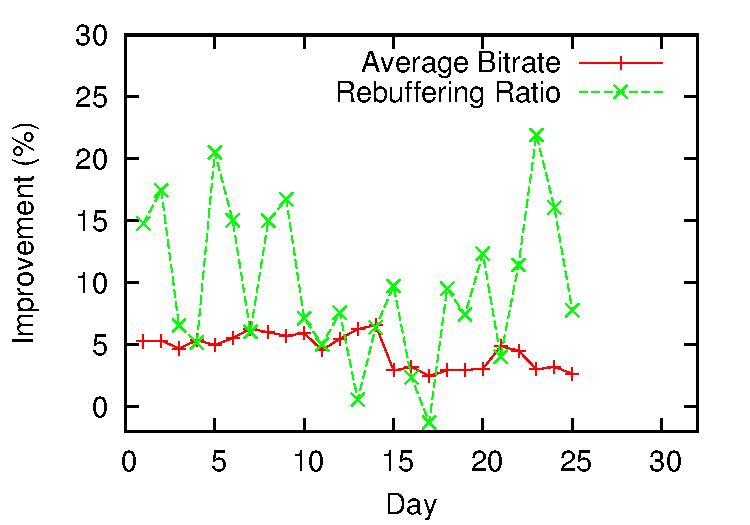
\includegraphics[width=0.25\textwidth, angle=270] {figures/eval-perfimp.pdf}
\tightcaption{Performance Improvement Using GO}
\label{fig:perf-impr}
\end{figure}


\tightsubsection{Adaptive Bitrate Stability}

\tightsubsubsection{When Do Bitrate Switching Happen?}

In this section, we empirically study when do bitrate switching happen. Figure~\ref{fig:switch-time-dist} shows when adaptive bitrate switch happen, where
x-axis is the percentage of actual video play time instead of content length. This is a conservative approach.

It shows that the majority of switches happen at 
the beginning of the video plays, i.e., X of the switches happen within Y of the video duration. 

\begin{figure}[h!]
\centering
 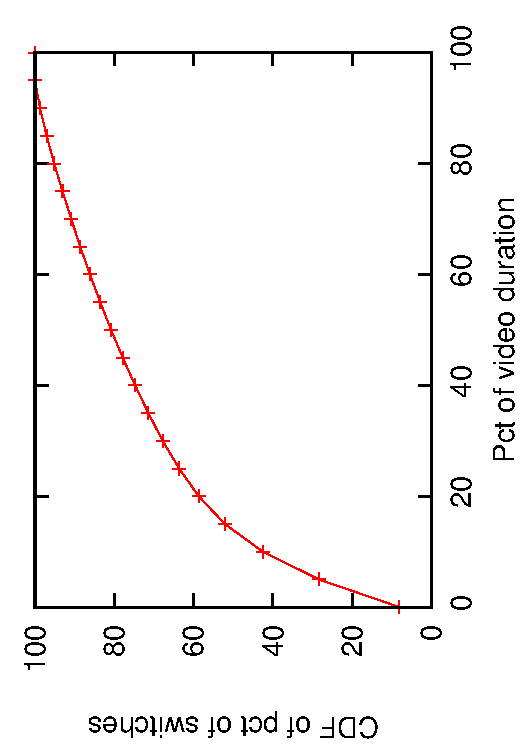
\includegraphics[width=0.25\textwidth, angle=270] {figures/switch-time-dist.pdf}
\tightcaption{Distribution of When Adaptive Bitrate Switches Happen}
\label{fig:switch-time-dist}
\end{figure}


\xil{we may add more algorithms if have time, also this may move from evaluation to previous sections since it is not really performance evaluation of algorithms.}

\tightsubsubsection{Reducing Number of Bitrate Switch}

Figure~\ref{fig:reduce-switch} shows the number of bitrate switches for optimized and random decisions within the first minute. 
It shows that GO can reduce the number of switches.

\begin{figure}[h!]
\centering
 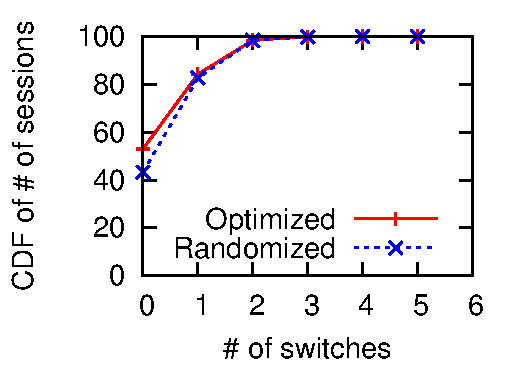
\includegraphics[width=0.25\textwidth, angle=270] {figures/eval-reduceswitch.pdf}
\tightcaption{Number of adaptive bitrate switches}
\label{fig:reduce-switch}
\end{figure}

\tightsubsubsection{Initial vs. Dominant Bitrate}

Figure~\ref{fig:initvsdom} shows the ratio of initial bitrate to dominant bitrate (1 is best). It shows that GO is close to dominant bitrate.

\begin{figure}[h!]
\centering
 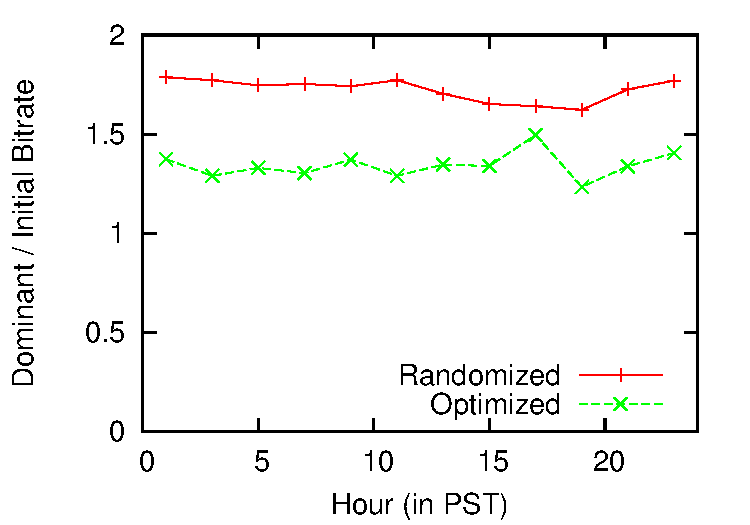
\includegraphics[width=0.25\textwidth, angle=270] {figures/eval-initvsdom.pdf}
\tightcaption{Dominant bitrate to initial bitrate}
\label{fig:initvsdom}
\end{figure}

